% !TEX root = diss.tex

\chapter{Methods}
\label{ch:methods}

In this chapter, we shall briefly outline the procedures and computational
methods used to obtain the results in this thesis. The methods have been broken
down in a per chapter manner. All quantum mechanical calculations were performed
using either the Gaussian 09\cite{Frisch2009} or TURBOMOLE
programs.\cite{turbomole} Molecular structures were built in the GaussView
program.\cite{gview} Optimised structures were verified local minima by
vibrational analysis and visualised using the Chemcraft program.\cite{ccraft}
Transition state structures were all verified saddle points by visualisation of
a single imaginary frequency connecting reactants to products. As a brief note
on notation, computational methods used are described using the following
notation: \emph{method}/\emph{basis}, for example, calculations performed using
the B3LYP density functional with 6-31+G* basis sets is denoted as
B3LYP/6-31+G*. Commonly, single-point energy calculations with a higher level of
theory (\emph{HL method} and \emph{HL basis}) are performed on structures
optimised with a lower level of theory (\emph{LL method} and \emph{LL basis}),
this is denoted as \emph{HL method}/\emph{HL basis}//\emph{LL method}/\emph{LL
  basis}. Thermochemical corrections are also taken from the lower level of
theory.

\section{Chapter \ref{ch:arrhenius}}

In this chapter, we seek to calculate pre-reaction complex binding energies for
bulky phenolic or peroxylic substrates which participate in nearly thermoneutral
reactions. Conformational analysis to locate the global minimum substrate
geometry was performed using the BLYP-D3(BJ)
method\cite{Becke1988,Lee1988,Grimme2010,Johnson2006} utilising the minimal
MINIs basis sets\cite{Huzinaga1984} and our groups own \emph{basis set
  incompletion potentials} (BSIPs).\jnote{citation needed} Geometries were
manipulated by manual rotation of the necessary dihedral bond angles, followed
by geometry optimisation and vibrational analysis.

The lowest energy substrates were combined to generate the appropriate
pre-reaction complexes. These pre-reaction complexes were subject to
conformational analysis using the same BLYP-D3(BJ)-BSIP/MINIs method. Geometries
were initially manipulated by hand. It became apparent that manual manipulation
resulted in an unsatisfactory exploration of the conformational space. To
overcome this, all the necessary dihedral angles were scanned systematically
using a combination of scripts.\cite{note5} All manipulated geometries were
subject to optimisation. For each complex, the top 5-10 complex geometries were
subject to further optimisation using a higher level of theory
(BLYP-D3(BJ)/pc-1) to obtain the final minimum energy pre-reaction complex
structures.\jnote{currently some non-minimum structures}

To obtain accurate pre-reaction complex binding energies, the substrates and
complexes were subject to single-point energy calculations using the
LC-$\omega$PBE long-range corrected density
functional\cite{Vydrov2006,Vydrov2006a} with D3(BJ) dispersion corrections and
pc-2 basis sets with truncated $f$-type functions (pc-2-spd).\cite{Johnson2013}
This method was selected on the recommendation of work by \citet{Johnson2013},
which demonstrated that this was an efficient method for calculation NCIs with a
reasonable degree of accuracy.

\section{Chapter \ref{ch:bde}}

In this chapter, we probe the applicability of the Bell-Evans-Polanyi principle
in two broad classes of C-H bond hydrogen atom transfer reactions with \cumo. In
order to do this, we seek to calculate BDEs which are \emph{chemically
  accurate}, that is, within 1 \kcalmol of the ``true value.'' To achieve this,
the highly accurate W1BD\cite{Barnes2009} quantum mechanical composite method
was employed.

Unfortunately, some of the substrates of interest are too large to be treated
with the W1BD method, thus we sought a less computationally expensive method
which most gave results of comparable precision. There is currenly no literature
which benchmarks computational procedures for bond dissociation enthalpies. As a
consequence, we explored a variety of other quantum mechanical composite
methods, including: the G4 and G4(MP2) methods,\cite{Curtiss2007,Curtiss2007a}
and the CBS-QB3, ROCBS-QB3, and CBS-APNO
methods.\cite{Montgomery1999,Montgomery2000,Ochterski1996}

\jnote{Is the LDBS approach relevant if we didn't use it for analysus in the
  end?}  Additionally, we developed a method which we call the \emph{locally
  dense basis set approach} (LDBS), which makes use of the ROCCSD(T) method with
a basis set partitioning scheme. The partitioning scheme is as follows: groups
which are close the the bond being broken are treated with large basis sets
(pc-3), while groups which are further away have incrementally smaller basis
sets. Specifically, we use a 3/2/1 partitioning, such that the carbons centred
group where bond dissociation occurs, as well as the groups immediately
adjacent, are treated with the high-level pc-3 basis sets. The next groups over
are treated with the medium-level pc-2 basis sets. Any groups beyond this are
treated with the low-level pc-1 basis sets. This is illustrated in
\ref{fig:ldbs}.


\begin{figure}[htb]
  \centering
  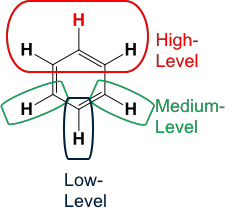
\includegraphics[width=0.6\textwidth]{figures/ldbs}
  \caption[Example locally dense basis set partitioning on benzene used in the
  LDBS approach.]{Example locally dense basis set partitioning on benzene used
    in the LDBS approach. The red hydrogen is that which is
    abstracted. High-level=pc-3, medium-level = pc-2, low-level = pc-1.}
  \label{fig:ldbs}
\end{figure}


The performance of all methods was compared to both the W1BD calculated BDEs, as
well as with experimentally available values, compiled from the \emph{Handbook
  of Bond Dissociation Energies}.\cite{Luo2002} Experimental values are obtained
using a wide variety of techniques, some of which may not be entirely
reliable. For example, thermochemical cycles\cite{Bordwell1988} are often used
to measure BDEs, however, this method has been shown to be unreliable if the
reaction used occurs by PCET rather than direct HAT.\cite{Miller2016} For this
reason, a secondary goal of this work is to identify any experimental BDEs which
may be in question.

To further probe the priniciples underlying the HAT reactions involved, TS
structures for the HAT reaction with \cumo have been obtained for a large number
substrates. TS structures were obtained using the B3LYP-D3(BJ)/6-31+G*
method. Where possible, TS structures were obtained for both a cisoid and
transoid conformation of the substrate/\cumo couple. Substrates and TS complexes
were subject to single-point energy calculations at the
LC-$\omega$PBE-D3(BJ)/6-311+G(2d,2p) level of theory to obtain more reliable
reaction barrier heights.

\section{Chapter \ref{ch:hat}}

In this chapter, we seek to understand the effects of non-redox active metal
cations of the hydrogen atom transfer reactions involving various organic
substrates with oxygen centred radicals. As shall be discussed in Chapter
\ref{ch:hat}, there is little literature which addresses the issue of
interactions between organic substrates and alkali and alkaline earth metals. To
address this, a benchmark study has been performed.

\subsection{Benchmark study of non-redox active metal cations with organic
  substrates}

The benchmark set shall be discussed in detail in Chapter \ref{ch:hat}. In order
to avoid erroneous charge transfer from the possible charge transfer involved in
cation-substrate interactions, conformational analysis was performed by manual
geometry manipulation using the LC-$\omega$PBE-D3(BJ)/6-31+G**
method.\cite{Johnson2013a} The most stable conformations of metal-substrate
complexes was subjected to higher-level optimisation at the
LC-$\omega$PBE-D3(BJ)/6-311+G(3df,3pd) level of theory.

Initially, binding energy for the metal-substrate complexes was calculated using
the full electron CCSD(T)/CBS approach, utilising two-point basis set
extrapolation with aug-pc-3 and aug-pc-4 basis sets. These results showed
systematic problems in the convergence of basis sets to the complete basis set
limit for the alkali and alkaline earth metals. To address this, the binding
energies were re-calculated using the full electron CCSD(T)-F12* explicitly
correlated approach\cite{Hattig2010} with Def2-QZVPPD basis sets.

A variety of DFT methods and basis sets were benchmarked against the
CCSD(T)-F12*/Def2-QZVPPD results (see Appendix \jnote{BLANK} for full
details). Single point energy calculations were performed on
LC-$\omega$PBE-D3(BJ)/6-311+G(3df,3pd) structures. The validity of these
structures was tested by re-optimisation with the three best performing DFT
methods relative to the benchmark data (M05-2X, BMK-D3(BJ), and $\omega$B97X-D
with large basis sets). The average root mean square deviation in geometry was
found to be onle 0.007-0.008 \AA ~for all three methods, thus validating the
structures. We elected to move forward using the M05-2X functional on the basis
of the results obtained from the benchmark study of metal cation-substrate
interactions, and the well described ability of M05-2X to accurately describe
HAT reactions involving oxygen centred radical.\cite{Galano2013}


\subsection{Effects of metal cations on hydrogen atom transfer barrier heights}



%%% Local Variables:
%%% mode: latex
%%% TeX-master: "diss"
%%% End:
